\chapter{Problemanalyse}
    \label{chapter:ProblemAnalysis}
    \section{\imperia}
    \section{\wordpress}
    \section{Klassifizierung der Inhalte einer Webseite}
        %\url{http://www.fernuni-hagen.de/KSW/portale/babw/service/}

        %\begin{figure}
        %    \centering
        %    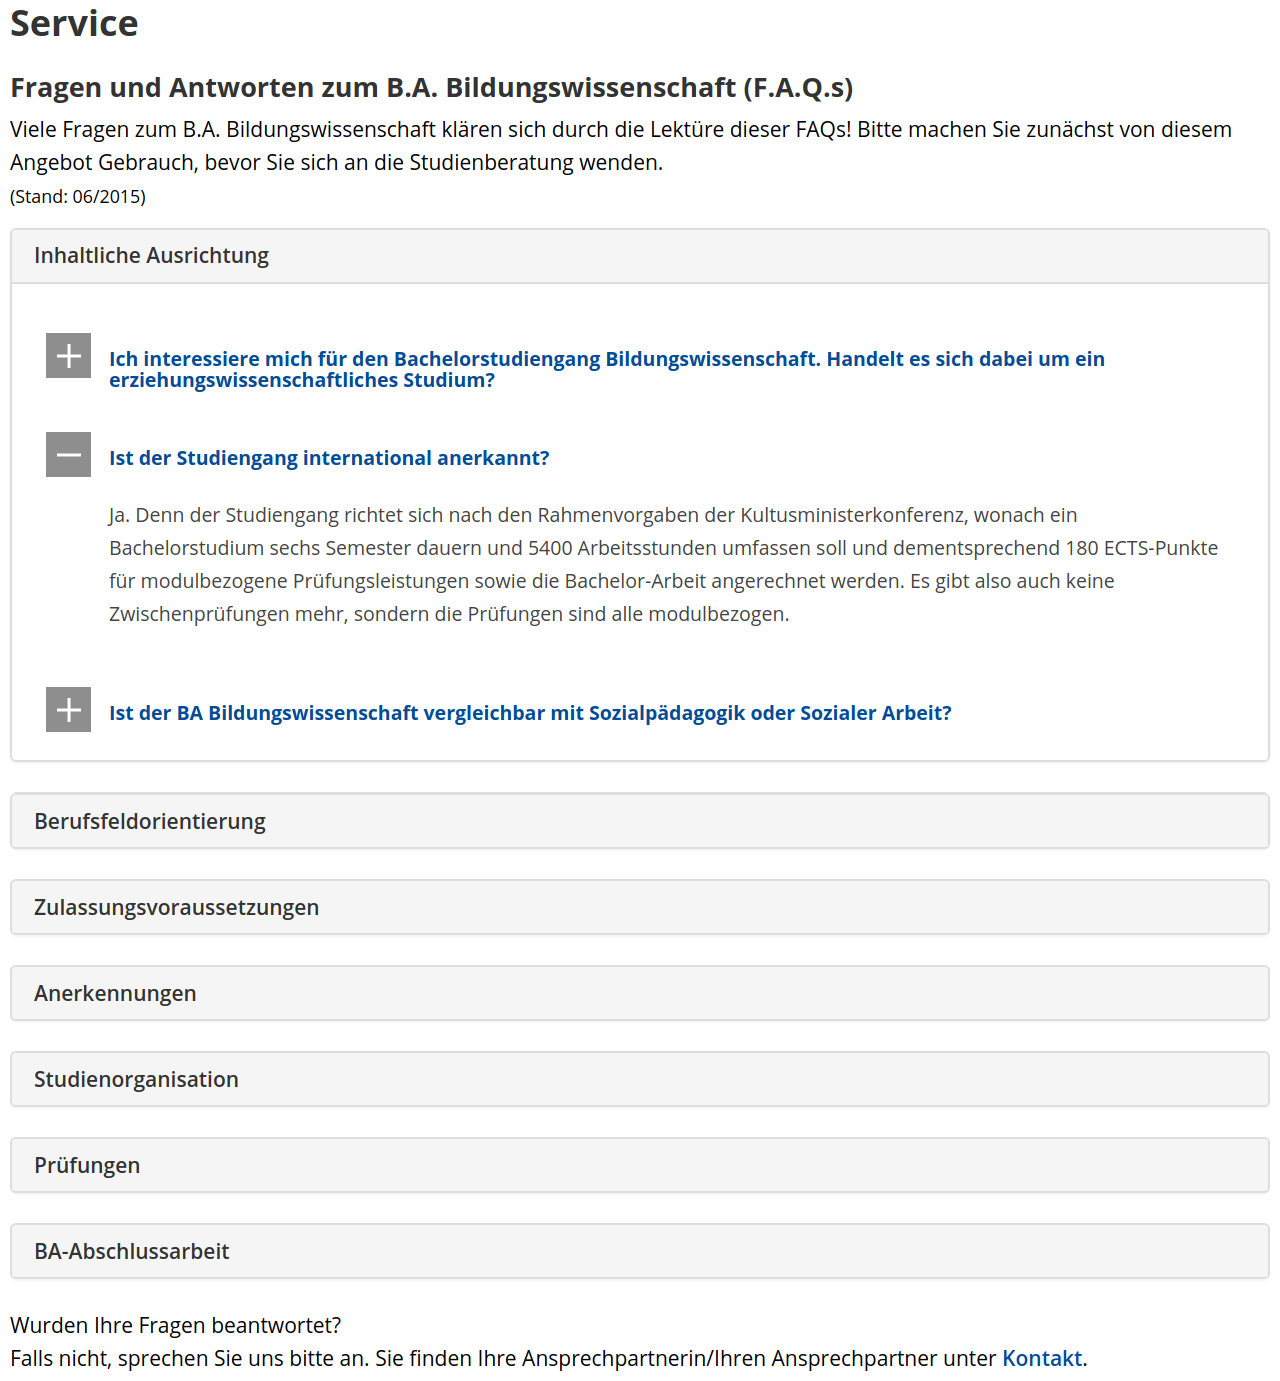
\includegraphics[width=\textwidth]{../resources/babw_service_faq.png}
        %    \caption{FAQ Seite des Studienportals B.A. Bildungswissenschaft}
        %    \label{image:BuildingBlocks}
        %\end{figure}
    
    \section{Das World Wide Web}
        Zur Lösung der beschriebenen Problemstellung ist eine genauere
        Betrachtung ihrer Domäne notwendig.
        Das Problem wird dadurch in einen größeren Kontext gesetzt,
        was zu einem besseren Verständnis und damit zur Findung
        einer geeigneten Lösung beiträgt.
        % TODO: Ref auf DDD?

        Die in diesem Fall zu betrachtende Domäne ist das "`\gls{www}"',
        welche das \gls{w3c} wie folgt definiert \cite{w3c:wwwArch}:

        \begin{quote}
            The \textit{\textbf{World Wide Web}} (\textit{\textbf{WWW}}, or simply \textit{\textbf{Web}})
            is an information space in which the items of interest, referred to as resources,
            are identified by global identifiers called Uniform Resource Identifiers (\textit{\textbf{URI}}).
        \end{quote}

        Diese Problemdomäne wird im Folgenden aus zwei Perspektiven betrachtet:
        Zunächst wird die Sicht eines Webseitenbesuchers auf das \gls{www} beschrieben.
        Anschließend stehen die konzeptionellen und technischen Grundlagen
        des \gls{www} im Vordergrund.
        Zusammen vermitteln diese Erläuterungen hinreichendes Wissen,
        um eine Lösung für die gegebene Problemstellung zu erarbeiten.

        \subsection{Das World Wide Web für Webseitenbesucher}
            Die Sicht eines Webseitenbesuchers (im Folgenden auch "`Endnutzer"' genannt)
            auf das \gls{www} ist simpel und sollte von jedem Leser nachvollzogen werden können.
            Dennoch bietet sie wichtige Einblicke.

            \paragraph*{Der Browser}
            Zugang zum \gls{www} erhält ein typischer Endnutzer über einen \textit{Browser}.
            In dessen Adresszeile trägt er einen \gls{url} ein,
            woraufhin der Browser die gewünschte Webseite lädt und anzeigt.
            Eine Webseite ist aus Sicht eines Endnutzers also eindeutig über eine
            Adresse, die allgemein "`URL"' oder "`Link"' genannt wird, gekennzeichnet.
            Der Browser dient zur Anzeige von Webseiten, wodurch er für Webseitenbesucher
            zu einem unentbehrlichen Werkzeug wird.
            Browser existieren für verschiedene Endgeräte,
            wie PCs, Smartphones und Tablets.
            Das heißt ein Webseitenbesucher ist an eine Form von Endgeräten gebunden.

            \paragraph*{Bestandteile}
            Sieht sich ein Besucher eine Webseite im Browser an,
            kann er schnell verschiedene Bestandteile ausmachen.
            Dazu zählen zunächst simple Elemente, mit denen er wenig bis gar nicht
            interagieren kann, also statischer Natur sind.
            Vertreter dieser Gruppe sind

            \begin{itemize}
                \item Texte,
                \item Bilder,
                \item Videos,
                \item Links auf andere Webseiten und
                \item Dateien, die zum Download bereitstehen.
            \end{itemize}

            Des Weiteren besitzt eine Webseite Designelemente,
            die in ihrem Aufbau oder ihrer Funktion komplexer
            als die zuvor genannten sind.
            Die Bibliothek Bootstrap\footnote{https://getbootstrap.com/}
            enthält zahlreiche solcher Komponenten.
            Beispielsweise bietet die Komponente "`Card"' die Möglichkeit
            Inhalte in komplexe Behälter einzubetten \cite{bootstrap:Cards}.
            Ein anderes Beispiel ist die Komponente "`Carousel"',
            welche der Erstellung von Diashows dient \cite{bootstrap:Carousel}.
            Letztere und viele weitere bieten dem Nutzer
            erweiterte Möglichkeiten zur Interaktion mit einer Webseite.

            Das gilt auch für Formular- oder Steuerelemente,
            die aus klassischen Applikationen bekannt sind,
            aber auch in Webseiten Anwendung finden.
            Dazu gehören unter anderem

            \begin{itemize}
                \item Textfelder,
                \item Schaltflächen,
                \item Dropdown-Listen,
                \item Checkboxen und
                \item Radiobuttons.
            \end{itemize}

            Allen Elementen ist gemein, dass ihr Aussehen sich von
            zwischen verschiedenen Webseiten unterscheiden kann.

            \paragraph{Varianten}
            Aus Sicht eines Endnutzers existieren oftmals mehrere
            Varianten derselben Webseite.
            Welche Variante er sieht hängt dabei von zwei Dimensionen ab:
            Sprache und Endgerät.

            Die heutige globalisierte und vernetzte Welt machen es oft erforderlich
            einen Internetauftritt auch auf internationele Besucher vorzubereiten.
            An erster Stelle bedeutet dies, dass Inhalte in verschiedene Sprachen
            übersetzt werden, um sie einem möglichst großen Publikum zugänglich zu machen.
            Für einen Endnutzer gibt es prinzipiell zwei Methoden,
            wie er eine Seite in seiner favorisierten Sprache anzeigen kann:

            \begin{itemize}
                \item   Die Webseite bietet ihm ein Steuerelement,
                        über das er selbst eine Sprache auswählen kann.
                \item   Die Webseite ermittelt automatisch die geeignete Sprache,
                        anhand verschiedener Parameter, die für den Besucher nicht zwangsläufig
                        offensichtlich sind.
            \end{itemize}

            Die Popularität mobiler Endgeräte wie Smartphones und Tablets
            bewegt immer mehr Betreiber von Webseiten dazu,
            verschiedene Versionen ihres Internetauftrittes anzubieten,
            die für verschiedene Geräte optimiert sind.
            Aus Sicht eines Besuchers gibt es bis zu drei geräteabhängige
            Varianten einer Webseite. Zwei für die oben genannten mobilen Geräte
            sowie eine weitere für PCs.
            Für ihn sind dabei drei Unterscheidungsmerkmale dieser Varianten offensichtlich:
            Inhalt, Design und Funktionalität.
            Ziel jeder Maßnahme ist es die Anzeigefläche,
            die ein Endgerät bietet, sinnvoll zu nutzen.
            Je kleiner ein Gerät ist, desto geringer ist diese Fläche,
            weshalb Inhalte auf kleineren Geräten weggelassen oder anderes
            dargestellt werden.
            Genauso können gewisse Funktionen einer Webseite nicht gleich
            gut sowohl auf großen PC- als auch auf kleinen Smartphone-Displays
            umgesetzt werden, ohne Anpassungen vorzunehmen.
            
            \paragraph*{Webanwendungen}
            Kapitel \ref{section:ContentManagementAndDesign} hat bereits
            kurz aufgezeigt, wie sich Webseiten stets weiterentwickeln.
            Ein wichtiger Aspekt dieser Weiterentwicklung ist aus Sicht
            eines Webseitenbenutzers, wie stark er mit ihr interagieren kann,
            was schon im Abschnitt über die Bestandteile einer Seite kurz aufgegriffen wurde.

            Angefangen bei simplen Seiten,
            die ursprünglich lediglich dazu gedacht waren Informationen
            bereitzustellen und mit anderen zu
            verlinken \cite{bernersLee:InformationManagement},
            entwickelten sich Webseiten im Laufe der Zeit weiter
            und boten immer mehr Möglichkeiten mit dem Nutzer zu interagieren
            und auf seine Aktionen zu reagieren.
            Folglich hielten immer mehr Merkmale klassischer Computeranwendungen
            Einzug in Webseiten.
            Heute stehen Webseiten klassischen Applikationen in Nichts nach,
            weshalb mit ihnen auch komplexe Anwendungen umgesetzt werden.
            Ein gutes Beispiel hierfür sind Googles Office-Anwendungen
            Docs\footnote{\url{https://www.google.com/intl/de/docs/about/}},
            Sheets\footnote{\url{https://www.google.com/intl/de/sheets/about/}},
            und Slides\footnote{\url{https://www.google.com/intl/de/slides/about/}},
            die in der Lage sind in vielen Fällen klassische Office-Anwendungen zu ersetzen.
            Aufgrund dieses besonderen Charakters ist für solche Webseiten auch der Begriff
            "`Webanwendung"' gebräuchlich.

            Im Vergleich zu herkömmlichen Anwendungen besitzen Webanwendungen zwei wichtige Vorteile.
            Solange man einen Internetzugang hat, sind sie zu jeder Zeit und von jedem Ort aus nutzbar.
            Des Weiteren können sie auf jedem Gerät ausgeführt werden,
            das einen Browser besitzt. Wie zuvor beschrieben ist dies nicht mehr ausschließlich ein PC,
            sondern auch mobile Endgeräte wie Smartphones und Tablets.

            \paragraph*{Websites}
            Der Internetauftritt einer Organisation besteht selten aus einer
            einzelnen Webseite.
            Stattdessen besteht er aus vielen Webseiten,
            die untereinander verlinkt sind und von der jede einen eigenen
            \gls{url} besitzt.
            Neben "`Internetauftritt"' hat sich der Begriff "`Website"' zur
            Referenzierung dieser Gesamtheit aller Webseiten einer Organisation
            etabliert \cite{duden:Internetauftritt, oxford:Website}.

            \paragraph*{Klassifizierung}
            Basierend auf ihrer primären Funktion lassen sich Webseiten grob klassifizieren.
            Die Bezeichnungen der resultierenden Klassen finden sich häufig im Sprachgebrauch
            von Webseitenbesucher wieder.

            Als \textit{Suchmaschinen} werden beispielsweise häufig die Seiten
            \url{https://www.google.de} und \url{https://www.bing.com/} bezeichnet.
            Andere geläufige Klassen sind:

            \begin{itemize}
                \item Online-Shops,
                \item Blogs,
                \item Homepages (Internetauftritt einer Organisation oder Privatperson),
                \item Social Networks
                \item Wikis
            \end{itemize}

            Eine weitere Kategorie sind die bereits erörterten Webanwendungen,
            also Webseiten, die bewusst als Oberflächen vob Anwendungen wahrgenommen werden.

            Viele Webseiten können unterschiedlich klassifiziert werden.
            Jede Suchmaschine und jeder Online-Shop ist gleichzeitig auch eine
            Webanwendung. Wie am Anfang dieses Abschnittes erwähnt ist für die
            Klassifizierung aus Endnutzersicht aber die primäre Funktion einer Webseite
            relevant.

        \subsection{Konzeptionelle und technische Grundlagen}